\begin{figure}[htbp]
\centering
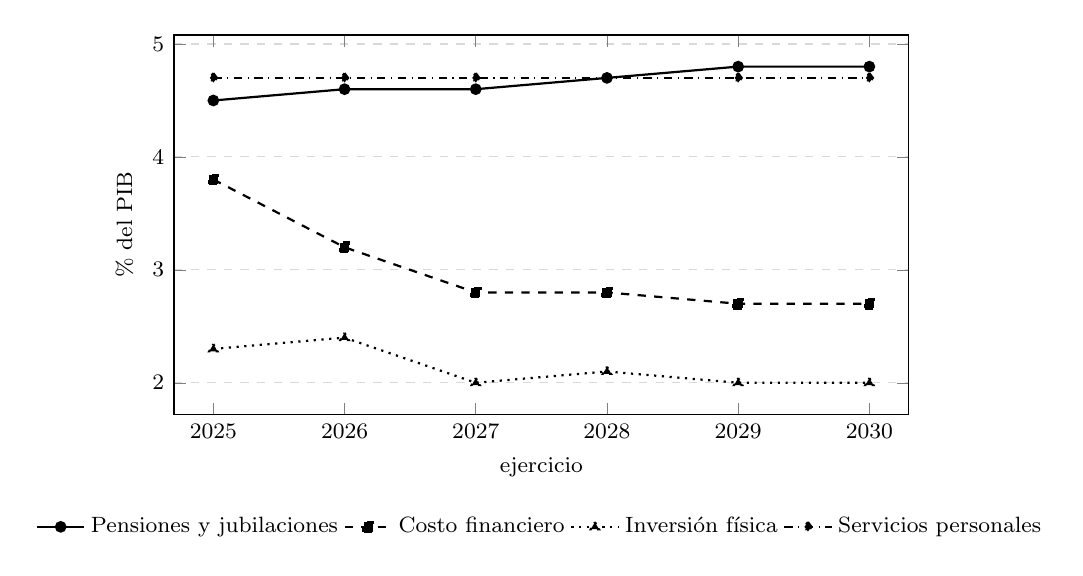
\begin{tikzpicture}
\begin{axis}[
  width=0.9\textwidth, height=6.4cm,
  xlabel={ejercicio}, ylabel={\% del PIB},
  legend style={font=\footnotesize, at={(0.5,-0.24)}, anchor=north,
                 legend columns=-1, draw=none},
  tick label style={font=\footnotesize},
  label style={font=\footnotesize},
  x tick label style={/pgf/number format/1000 sep={}},
  ymajorgrids=true, grid style={dashed, gray!30},
  enlarge x limits=0.06,
  cycle list={{solid,mark=*}, {dashed,mark=square*}, {dotted,mark=triangle*}, {dashdotted,mark=diamond*}},
  xtick=data,
]
\addplot+[thick, mark size=1.7pt] coordinates {(2025,4.5) (2026,4.6) (2027,4.6) (2028,4.7) (2029,4.8) (2030,4.8)};
\addlegendentry{Pensiones y jubilaciones}
\addplot+[thick, mark size=1.7pt] coordinates {(2025,3.8) (2026,3.2) (2027,2.8) (2028,2.8) (2029,2.7) (2030,2.7)};
\addlegendentry{Costo financiero}
\addplot+[thick, mark size=1.7pt] coordinates {(2025,2.3) (2026,2.4) (2027,2.0) (2028,2.1) (2029,2.0) (2030,2.0)};
\addlegendentry{Inversión física}
\addplot+[thick, mark size=1.7pt] coordinates {(2025,4.7) (2026,4.7) (2027,4.7) (2028,4.7) (2029,4.7) (2030,4.7)};
\addlegendentry{Servicios personales}
\end{axis}
\end{tikzpicture}
\caption{Gasto por clasificación económica en el escenario oficial, 2025--2030}
\label{fig:F12_2}
\par\vspace{2pt}\footnotesize Fuente: elaboración propia del ITED con información de la SHCP, CGPE 2025, Anexo III.2, p. 85. Pensiones es la única de las cuatro que sube. El CGPE 2025 se publicó sin capa de texto; las cifras se leyeron de la página renderizada y se validaron por identidad contable.
\end{figure}
